% assignment_3.tex
% CS 8725 - Supervised Learning (Fall 2015)
%     University of Missouri-Columbia
%             Chanmann Lim
%            September 2015

\documentclass[a4paper]{article}

\usepackage[margin=1 in]{geometry}
\usepackage{listings}
\usepackage{amsmath}
\usepackage{amsfonts}
\usepackage{graphicx}
\usepackage{float}
\usepackage{multirow}

\everymath{\displaystyle}
\DeclareMathOperator*{\argmax}{\arg\!\max}
\DeclareMathOperator*{\argmin}{\arg\!\min}

\begin{document}
\title{CS 8725: Report for assignment 3}
\author{Chanmann Lim}
\date{September 28, 2015}
\maketitle

\noindent
	The Matlab code for all experiments is in the \textbf{Appendix} section.

\paragraph{Programming 1:} We are given a bunch of data samples of "Average height and weight of American women aged 30 to 39" and the task is to design linear regression algorithm to predict the $ weight \in \mathbb{R}$ denoted by $Y$ from a given height measurement denoted by $X$ then the problem becomes $f(X) \to Y$ finding a function mapping from X to Y. In linear regression we assume that $f(X)$ take a linear form with respect to $X$ that is $f(X) = \beta_1 + \beta_2X$ and the goal is to choose $\hat{f}(X)$ that minimizes the prediction error (squared error). \\

	\begin{equation}
		\hat{f}_n^L = \argmin_f \frac{1}{n} \sum_{i=1}^n (f(X_i) - Y_i)^2
	\end{equation}

	By rewriting $f(X)$ in term of $\beta = [\beta_1\; \beta_2]^T$, minimizing $f(X)$ becoming minimizing $\beta$.
	
	\begin{align}
		\hat{\beta} &= \argmin_{\beta} \frac{1}{n} \sum_{i=1}^n (X_i\beta - Y_i)^2\\
			&= \argmin_{\beta} \frac{1}{n} (A\beta - Y)^T(A\beta - Y)  \label{eq:beta_hat}
	\end{align}
	
	Where, 
	
	\begin{equation}
		A = \begin{bmatrix} 
				1 & X_1 \\ 
				\vdots & \vdots \\ 
				1 & X_n 
			\end{bmatrix} \text{ and }
		Y = \begin{bmatrix} 
				Y_1 \\ 
				\vdots \\ 
				Y_n 
			\end{bmatrix}
	\end{equation}
	
	If we define $J(\beta) = (A\beta - Y)^T(A\beta - Y)$ then minimizing $J(\beta)$ is equivalent to \eqref{eq:beta_hat}.
	
	\begin{align}
		\frac{\partial J(\beta)}{\partial \beta} &= \frac{\partial A^TA\beta\beta^T - 2\beta^TA^TY - Y^TY}{\partial \beta} \\ 
			&= 2A^TA\beta - 2A^TY
	\end{align}
	
	\begin{align}
		2A^TA\hat{\beta} - 2A^TY &= 0 \\ 
		A^TA\hat{\beta} &= A^TY \\ 
		\hat{\beta} &= (A^TA)^{-1}A^TY \label{eq:normal_eq}
	\end{align}
	
	Eq. ~\eqref{eq:normal_eq} is the normal equation with $(A^TA)$ as normal matrix and $\hat{f}_n^L = X\hat{\beta}$. As a result we obtained the linear regression coefficient in \eqref{eq:beta_hat_value} and the expected error in \eqref{eq:risk_1}:
	
	\begin{equation} \label{eq:beta_hat_value}
		\hat{\beta} = [-39.0620 \quad 61.2722]^T
	\end{equation}
	
	\begin{align}
		R(\hat{f}) &= \mathbb{E}[(\hat{f}(X) - Y)^2] \\ 
			&= \frac{1}{n} (X\hat{\beta} - Y)^T(X\hat{\beta} - Y) \\
			&= 0.4994 \label{eq:risk_1}
	\end{align}
	
	In fact for this case in particular, we know that we could further reduce the expected error $R(\hat{f})$ by introducing quadratic term into the regression. With this procedure we have turned linear regression into polynomial regression and by following the derivation in solving for $\hat{\beta}$ it turn out that $\hat{\beta} = (A^TA)^{-1}A^TY$ where $\beta = [\beta_1\;\beta_1\;\beta_3]^T$ and 
	$$ A = \begin{bmatrix} 
				1 & X_1 & X_1^2 \\ 
				\vdots & \vdots & \vdots \\ 
				1 & X_n & X_n^2
			\end{bmatrix}$$
			
	We obtained $\hat{\beta} = [128.8128 \quad -143.1620 \quad 61.9603]^T$ and $R(\hat{f}) = 0.0506$ for second order polynomial regression. Figure ~\ref{fig:regression} show the both linear and polynomial regression functions with respect to the data samples.
	
	\begin{figure}[H]
		\centering
		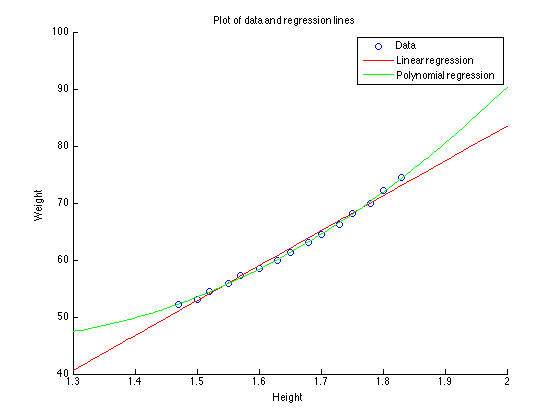
\includegraphics[scale=.57]{images/regression.png}
		\caption{Plot of data and regression lines}
		\label{fig:regression}
	\end{figure}
	
\paragraph{Programming 2:} In this task we are going to implement logistic regression classifier using iterative algorithm namely \textbf{gradient ascent} and test it on the Iris plant dataset by R.A Fisher available in UCI machine learning repository. The dataset consists of four features such as \emph{sepal length in cm}, \emph{sepal width in cm}, \emph{petal length in cm} and \emph{petal width in cm} and the class label. There are 50 instances from each class which make it a total of 150 samples however we are only interested in binary classification of \emph{Iris-Setosa} and \emph{Iris-Versicolor}, the other class \emph{"Iris-Virginica"} were removed from the dataset in the pre-processing phase. In addition we understand that \emph{Iris-Setosa} class is linearly separable from \emph{Iris-Versicolor}. \\ 

	In logistic regression, instead of trying to learn the likelihood probability $P(X|Y)$ it aims at learning $P(Y|X)$ the conditional likelihood directly from the data. And for binary classification the assumption is that:
	
	\begin{align}
		P(Y=0|X,w) &= \frac{1}{1+exp(w_0 + \sum_{i=1}^{d} w_iX_i)} \\ 
		P(Y=1|X,w) &= \frac{exp(w_0 + \sum_{i=1}^{d} w_iX_i)}{1+exp(w_0 + \sum_{i=1}^{d} w_iX_i)}
	\end{align}
	
	Henceforth, the job is find the optimal $\hat{\mathbf{w}}$ that maximizes the posterior probability.
	
	\begin{equation}
		\hat{\mathbf{w}} = \argmax_{\mathbf{w}} \prod_{j=1}^n P(Y^{(j)}|X^{(j)},\mathbf{w})
	\end{equation}
	
	From i.i.d assumption we have $p(D|\mathbf{w}) = \prod_{j=1}^{n} p(y^j|x^j,\mathbf{w})$. Since $y \in \{0, 1\}$ we can rewrite $p(D|\mathbf{w})$ as:
	
	\begin{align}
		p(D|\mathbf{w}) &= \prod_{j=1}^n p(y^j=1|x^j,\mathbf{w})^{y^j}p(y^j=0|x^j,\mathbf{w})^{1-y^j} \\ 
			&= \prod_{j=1}^n \left(\frac{exp(w_0+\sum_i w_ix_i^j)}{1+exp(w_0+\sum_i w_ix_i^j)}\right)^{y^j}\left(\frac{1}{1+exp(w_0+\sum_i w_ix_i^j)}\right)^{1-y^j}
	\end{align}
	
	\begin{equation}
		l(\mathbf{w}) = ln\;p(D|\mathbf{w}) = \sum_{j=1}^n \left[y^j(w_0+\sum_i^d w_ix_i^j)-ln(1+exp(w_0+\sum_i^d w_ix_i^j))\right]
	\end{equation}
	
	Then maximizing $l(\mathbf{w})$ the conditional log likelihood with respect to all elements of $\mathbf{w}$.
	
	\begin{align}
		\frac{\partial l(\mathbf{w})}{\partial w_i} &= \sum_{j=1}^n \left[y^jx_i^j - \frac{exp(w_0+\sum_i w_ix_i^j)}{1+exp(w_0+\sum_i w_ix_i^j)}x_i^j\right] \\ 
			&= \sum_{j=1}^n \left[x_i^j(y^j - p(y^j=1|x_i^j, \mathbf{w})\right]
	\end{align}
	
	The issue here is that there is no closed-form solution to solve for $\mathbf{w}$ directly, yet $l(\mathbf{w})$ is a concave function which will lead to converge at the global maximum by applying any optimization technique such as \textbf{gradient ascent} or newton's methods, etc,. \\
	
	\textbf{Gradient Ascent: } we started by initializing $\mathbf{w} = [w_0\; w_1\; w_2\; w_3\; w_4\; w_5]^T$ randomly between [-1, 1] then iteratively compute the gradient 
	$ \nabla_{\mathbf{w}} l(\mathbf{w}) = \left[
		\frac{\partial l(\mathbf{w})}{\partial w_0}, \cdots, 
		\frac{\partial l(\mathbf{w})}{\partial w_5}
	\right]^T$ and update $\mathbf{w}$ until a fixed number of iterations $T = 100000$ or stop when it converge.
	
	\begin{align}
		w_i^{(t+1)} &\leftarrow w_i^{(t)} + \alpha \frac{\partial l(\mathbf{w})}{\partial w_i} \\
			&= w_i^{(t)} + \alpha \sum_{j=1}^n x_i^j(y^j - p(y^j=1|x_i^j, \mathbf{w})
	\end{align}
	
	Where $w_i^{(t)}$ is the weight for $i^{th}$ component at iteration $t$ and $\alpha$ is the learning rate for which we chose $\alpha = 0.001$. And here we defined the convergence criteria as the percentage change of the conditional log likelihood $l(\mathbf{w})$ to be less then 0.03\% ($\epsilon = 0.0003$).
	
	\begin{equation}
		(\Delta \%l(\mathbf{w}) < \epsilon) \to \text{converge}
	\end{equation}
	
	We can see in Figure ~\ref{fig:gradient_ascent}. that the conditional log likelihood scores keep increasing and \textbf{gradient ascent} algorithm converge at $t=3022$ for the initialization of $\mathbf{w} = [-0.0665, -0.4920, -0.1376, 0.4051, -0.1953]^T$.
	
	\begin{figure}[H]
		\centering
		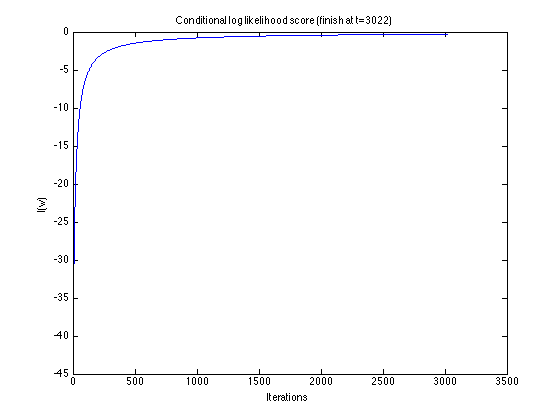
\includegraphics[scale=.57]{images/gradient_ascent.png}
		\caption{Plot of conditional log likelihood scores}
		\label{fig:gradient_ascent}
	\end{figure}
	
	To evaluate, we can compare and predict the class with higher posterior probability between $P(Y=0|X, \mathbf{w})$ and $P(Y=1|X, \mathbf{w})$ and decision boundary is
		
	\begin{align}
		\frac{P(Y=1|X, \mathbf{w})}{P(Y=0|X, \mathbf{w})} = 1 \\ 
		exp(w_0 + \sum_i^d w_iX_i) = 1 \\ 
		w_0 + \sum_i^d w_iX_i = 0
	\end{align}
	
	At this stage we understand that the decision boundary for logistic regression is simply a linear function and since the dataset we are working with for this experiment is linearly separable we expect our classifier to be able to perfectly predict the correct category of each samples. And the outcome yield 100\% training accuracy which is indeed consistent with our presumption.
	
	\begin{equation}
		accuracy = \frac{\sum_i^n \mathbf{1}_{predicted_i = Y_i}}{n}
	\end{equation}
	
\paragraph{Experimental:} ~\\

 	Choice of $\mathbf{w}^{(t=0)} = \mathbf{0}$ is not at all bad of a choice since we know that gradient ascent will converge due to the concavity of the function we are maximizing however good practices in general optimization procedure avoid this since it starts the optimization at $P(Y=0|X) = P(Y=1|X) = 0.5$ thus might be more likely to lead to local optima and get stuck than a randomly generated one. \\
	
	Choice of $\alpha$, the learning rate or step-size in gradient ascent algorithm, is used to control the penalized contribution of a particular $\mathbf{w}$ at each iteration. Although there is no rule of thumb in determining the right value for $\alpha$ other than the constraint that $\alpha \in [0,1]$, empirical successes suggested that given large enough number of iterations we could start with $\alpha = 1$ then keep tuning by decreasing to a factor of three (eg. $\alpha = \{1, 0.3, 0.1, 0.03, 0.01, \cdots \}$) and we found that $\alpha = 0.001$ give us smooth convergence comparing to other numbers. While smaller $\alpha$ make gradient ascent stop because either the change of $l(\mathbf{w})$ is not significant or it reached the pre-defined maximum iterations $T=100000$; larger $\alpha$ oscillated the value of $l(\mathbf{w})$ which we are trying to maximize if not diverge completely.
\newpage
\subsection*{Appendix:}
	\lstinputlisting[language=Matlab, title=\lstname, basicstyle=\footnotesize]{assignment_3.m}
	\lstinputlisting[language=Matlab, title=\lstname, basicstyle=\footnotesize]{problem_1.m}
	\lstinputlisting[language=Matlab, title=\lstname, basicstyle=\footnotesize]{problem_2.m}
\end{document}